%!TEX root = ../../main.tex

\section{Shields}
\subsection{Kar-shield}

Til at styre interaktion med karret implementeres følgende eksterne kredsløb, der alle køres fra karPsoC'en: 

\begin{description}
 \item[•] Indløbsventil
 \item[•] Afløbsventil
 \item[•] Doseringspumpe
 \item[•] RS-konverter til KarBus
 \item[•] RS-konverter til ØBus
 \item[•] Flowsensor
 \item[•] pH-probe
\end{description}
 
Det er valgt at benytte Shield-teknologi, så alle kredsløbene implementeres på samme print, som er kompatibel med PSoC4 pinlayout på Pioneerkittet. På denne måde kan det færdige print sættes direkte på Pioneerkittet, og alle pinconnections er dermed sikret internt de 2 boards imellem. 
Det er valgt at benytte PCB-layout programmet Eagle. Her benyttes pre-defineres biblioteker med komponenter til at opbygge de ønskede kredsløb og udlægge printbaner.  

\subsubsection{Oprettelse af egne komponenter} \hspace{0pt} \\
Dog er det ikke alle komponenter der kan findes, derfor kan det være nødvendig at oprette sige egne ud fra de ønskede komponenters datablade. 
For at kunne implementere det eksterne counterkredsløb på shield'et, er det nødvendigt at oprette en custom model af 74HC393-counteren, samt 74HZ08-gaten.
Dette skyldes at på de eksisterende modeller af disse moduler, er GND internt rout'ed, og således tænkt benyttet i forbindelse med et internt stelplan der benyttes på mange print. Men da der i vores tilfælde ønskes at kunne connecte GND fysisk til én af PSoC'ens GND-pins, skal dette kunne routes manuelt.
I Eagle oprettes der et brugerbibliotek, og deri en custommodel af modulerne med igangspunkt i databladene. (herunder ses oprettelse af HC393)
Først udlægges pins på IC'en, se fig.\ref{screenshot:EagleComponents} på s.\pageref{screenshot:EagleComponents}

\begin{figure}[H]
	\centering
	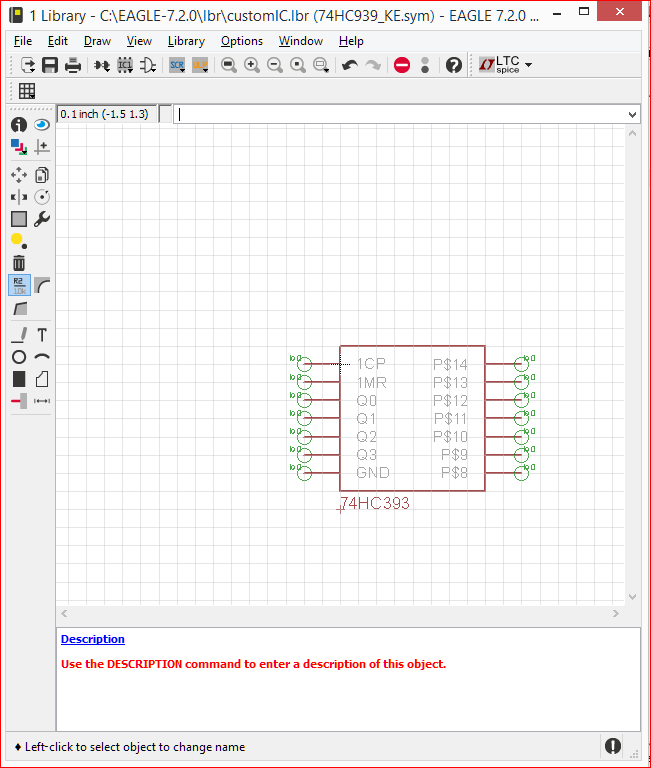
\includegraphics[scale=0.6]{../Hardware/Shields/Screenshots/OprettelseAfEgneKomponenter}
	\caption{Screenshot: Oprettelse af egne komponenter i Eagle}
	\label{screenshot:EagleComponents}
\end{figure}

Her hentes værdier fra databladet.

Derudover skal der oprettes et footprint til modellen så denne kan pleceres på printet. Her hentes Package outline-specs fra databladet. Da begge IC'er følger standard package mål, er afstanden imellem de 2 rækker 0.3 inches, og afstanden imellem hvert ben er 0.1 inches. 
Målene vælges i inches da Eagle benytter inches som standard. Værdierne ses dokumenteret herunder, fig.\ref{screenshot:PackageOutline} 

\begin{figure}[H]
	\centering
	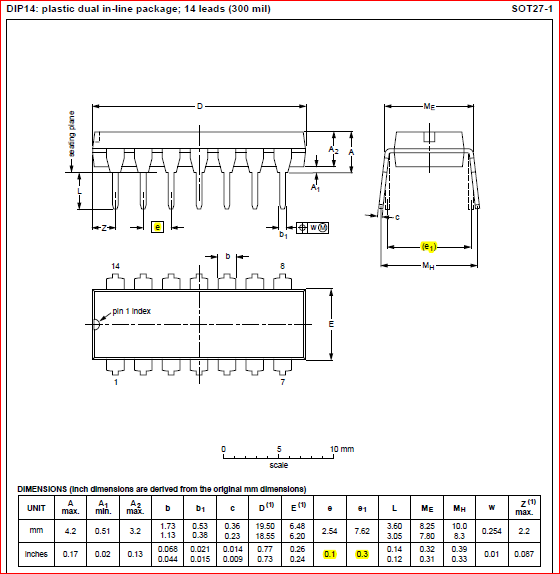
\includegraphics[scale=0.6]{../Hardware/Shields/Screenshots/PackageOutline}
	\caption{Screenshot: Package Outline fra databladets Fig.13, s-14 }
	\label{screenshot:PackageOutline}
\end{figure}

	
Disse værdier benyttes til at skabe følgende footprint, og dette mappes til pins fra schematic. 

\begin{figure}[H]
	\centering
	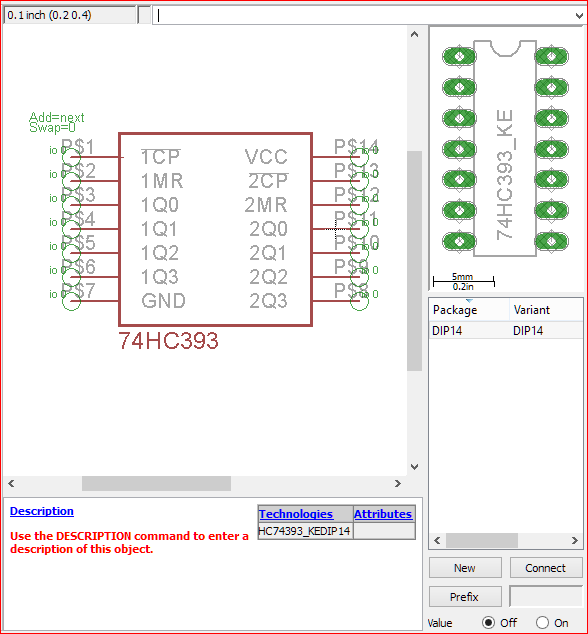
\includegraphics[scale=0.5]{../Hardware/Shields/Screenshots/Mapping}
	\caption{Screenshot: Mapping af pins}
	\label{screenshot:Mapping}
\end{figure}
	
Det samme foretages for AND-gate IC'en. 
Herefter kan modellerne indsættes på Kar-shield'et og herefter kan GND frit routes, som det ses på det færdige print, fig.\ref{screenshot:karShield}, s.\pageref{screenshot:karShield}.


\newpage
\begin{figure}[H]
	\centering
	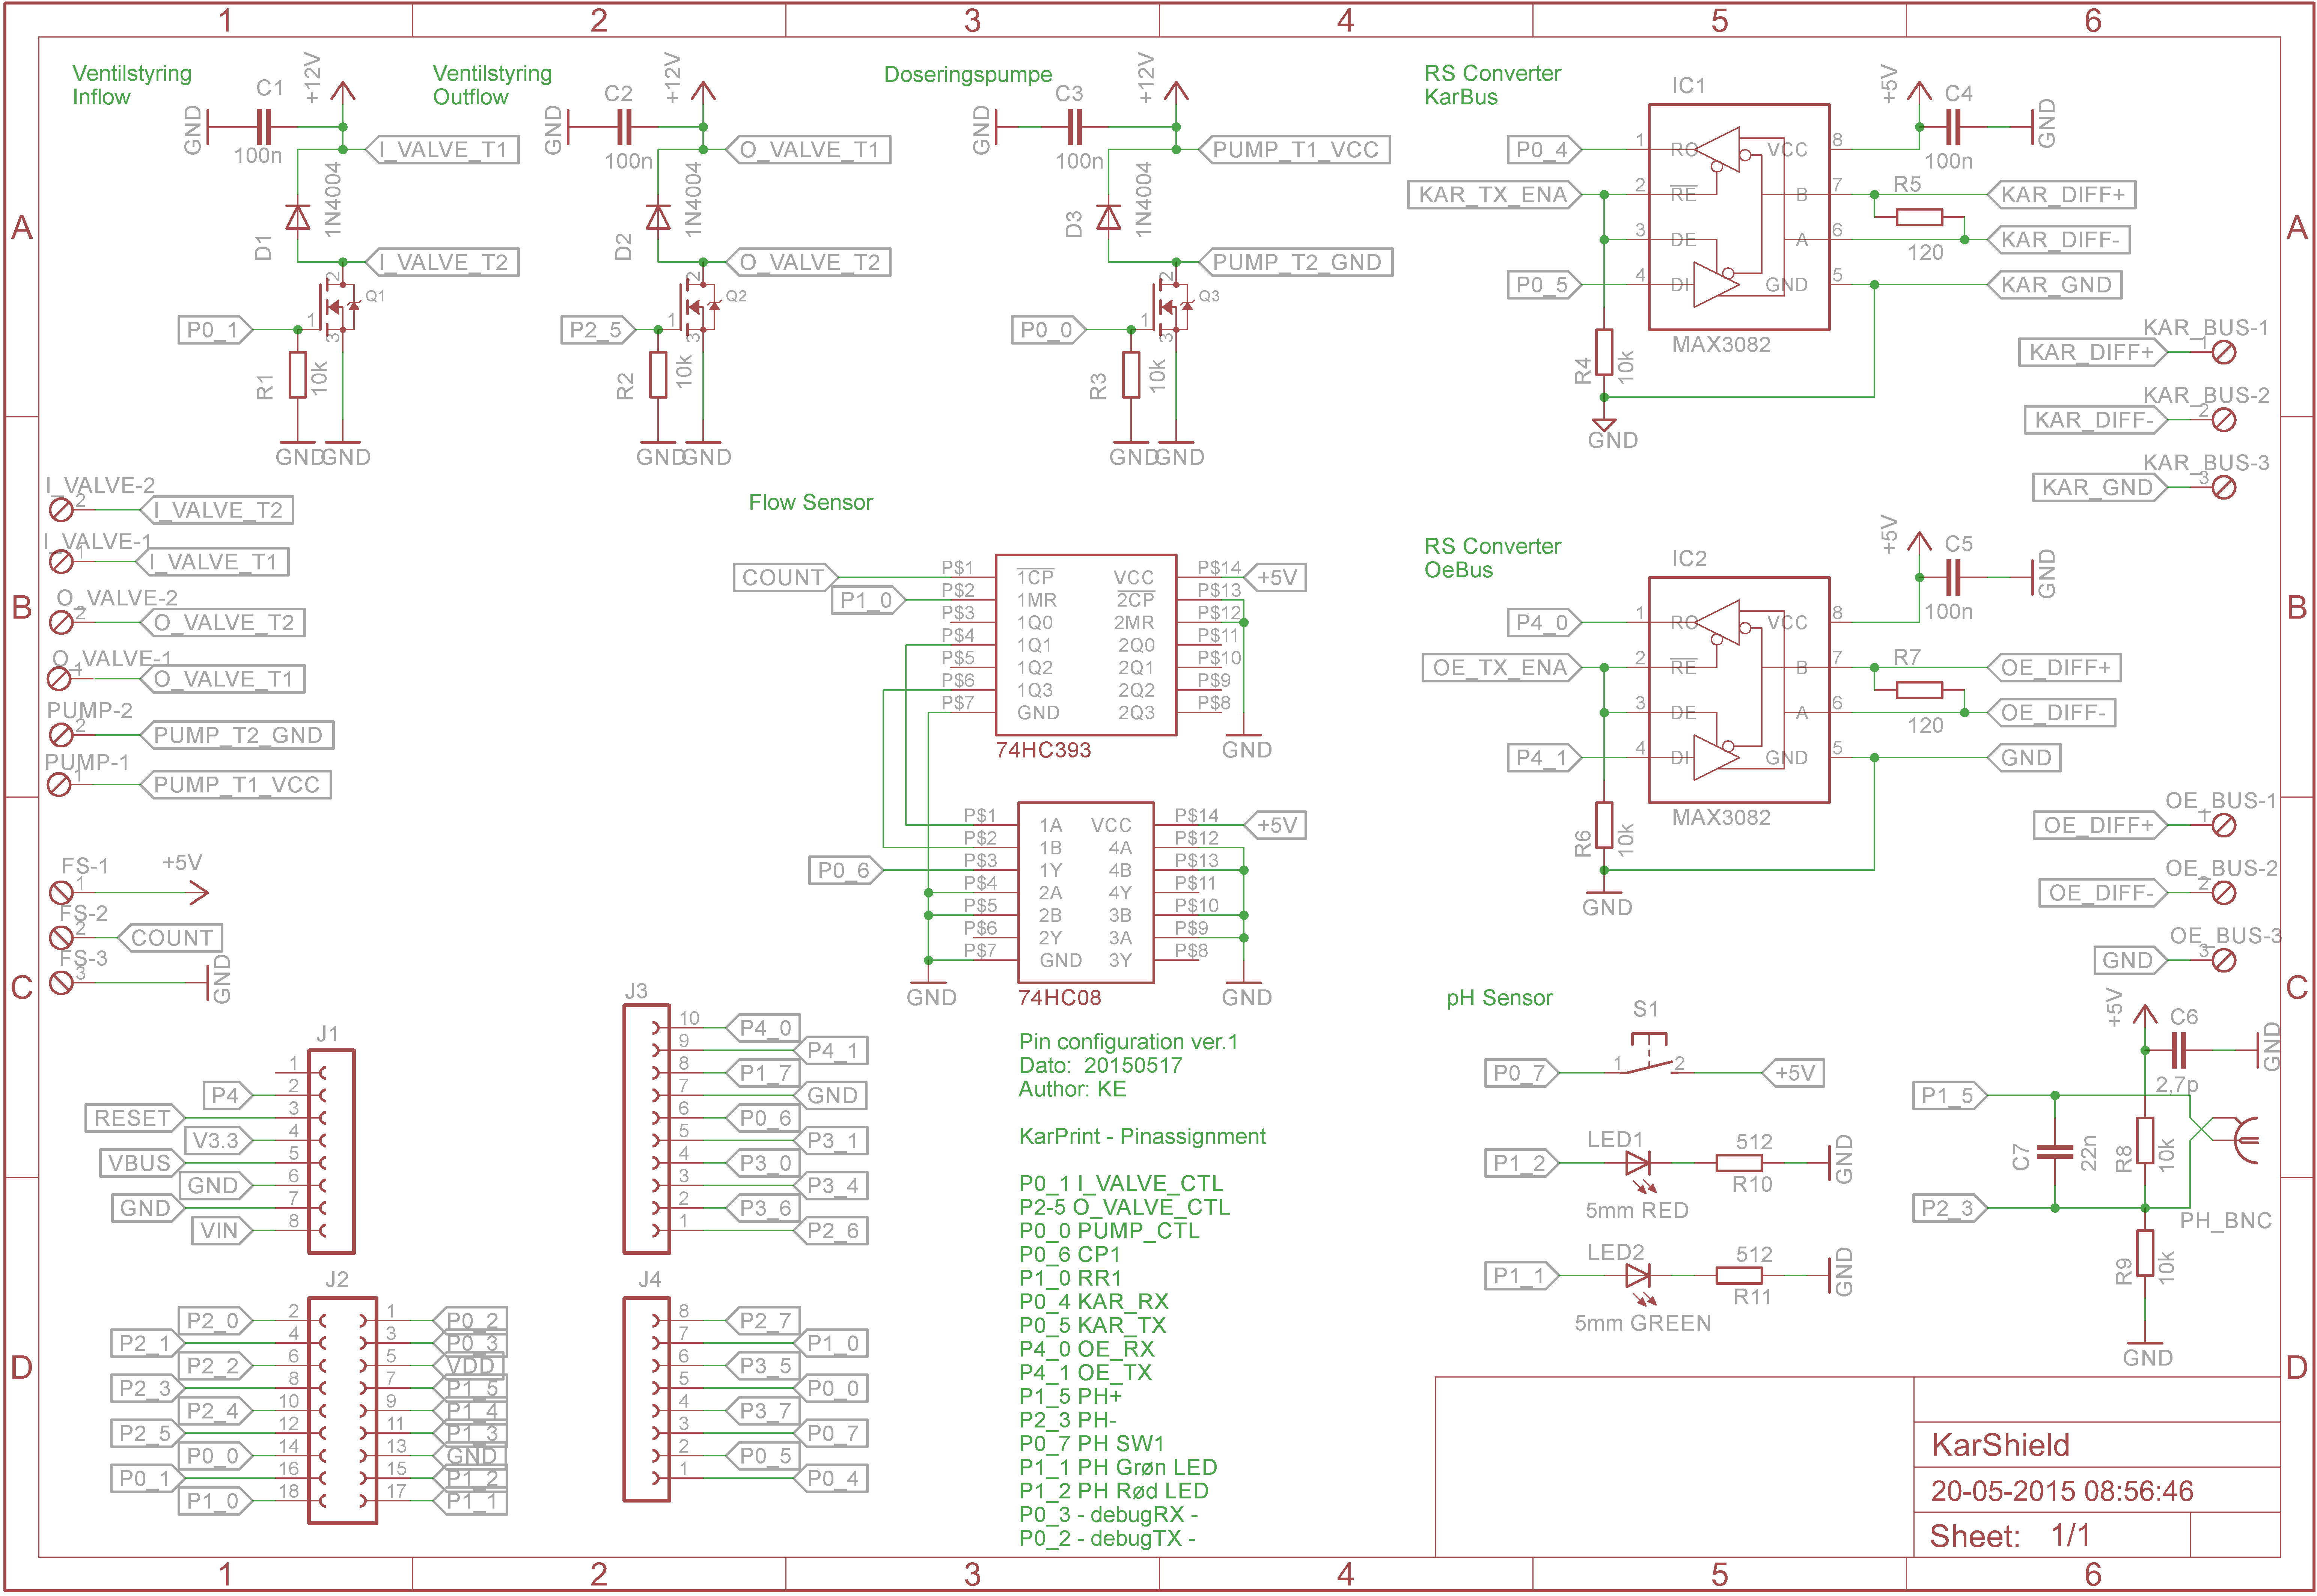
\includegraphics[scale=1]{../Hardware/Shields/Screenshots/KarShield}
	\caption{Screenshot: Det færdige KarShield}
	\label{screenshot:karShield}
\end{figure}

\fxnote{Siden med KarShield-diagram skal være A3}


\newpage
\subsection{Ø-shield}

På samme måde som karShield oprettes også et shield til sensor Ø'en. Dette shield indeholder følgende komponenter: 

\begin{description}
 \item[•] Doseringsventil
 \item[•] RS-konverter til ØBus
 \item[•] I2C Kommunikation til Jordfugt sensor
\end{description}

Her implementeres doseringsventilen, der kontrollere om dosering til gromediet er muligt. Derudover findes RS-konverter til Ø-bussen. Sidst findes I2C kommuniktation med jordfugtsensor-PSoC'en. 
Shield'et monteres på Ø-PSoC'en.

Det færdige print ses på fig.\ref{screenshot:OeShield}, s.\pageref{screenshot:OeShield}.

\newpage
\begin{figure}[H]
	\centering
	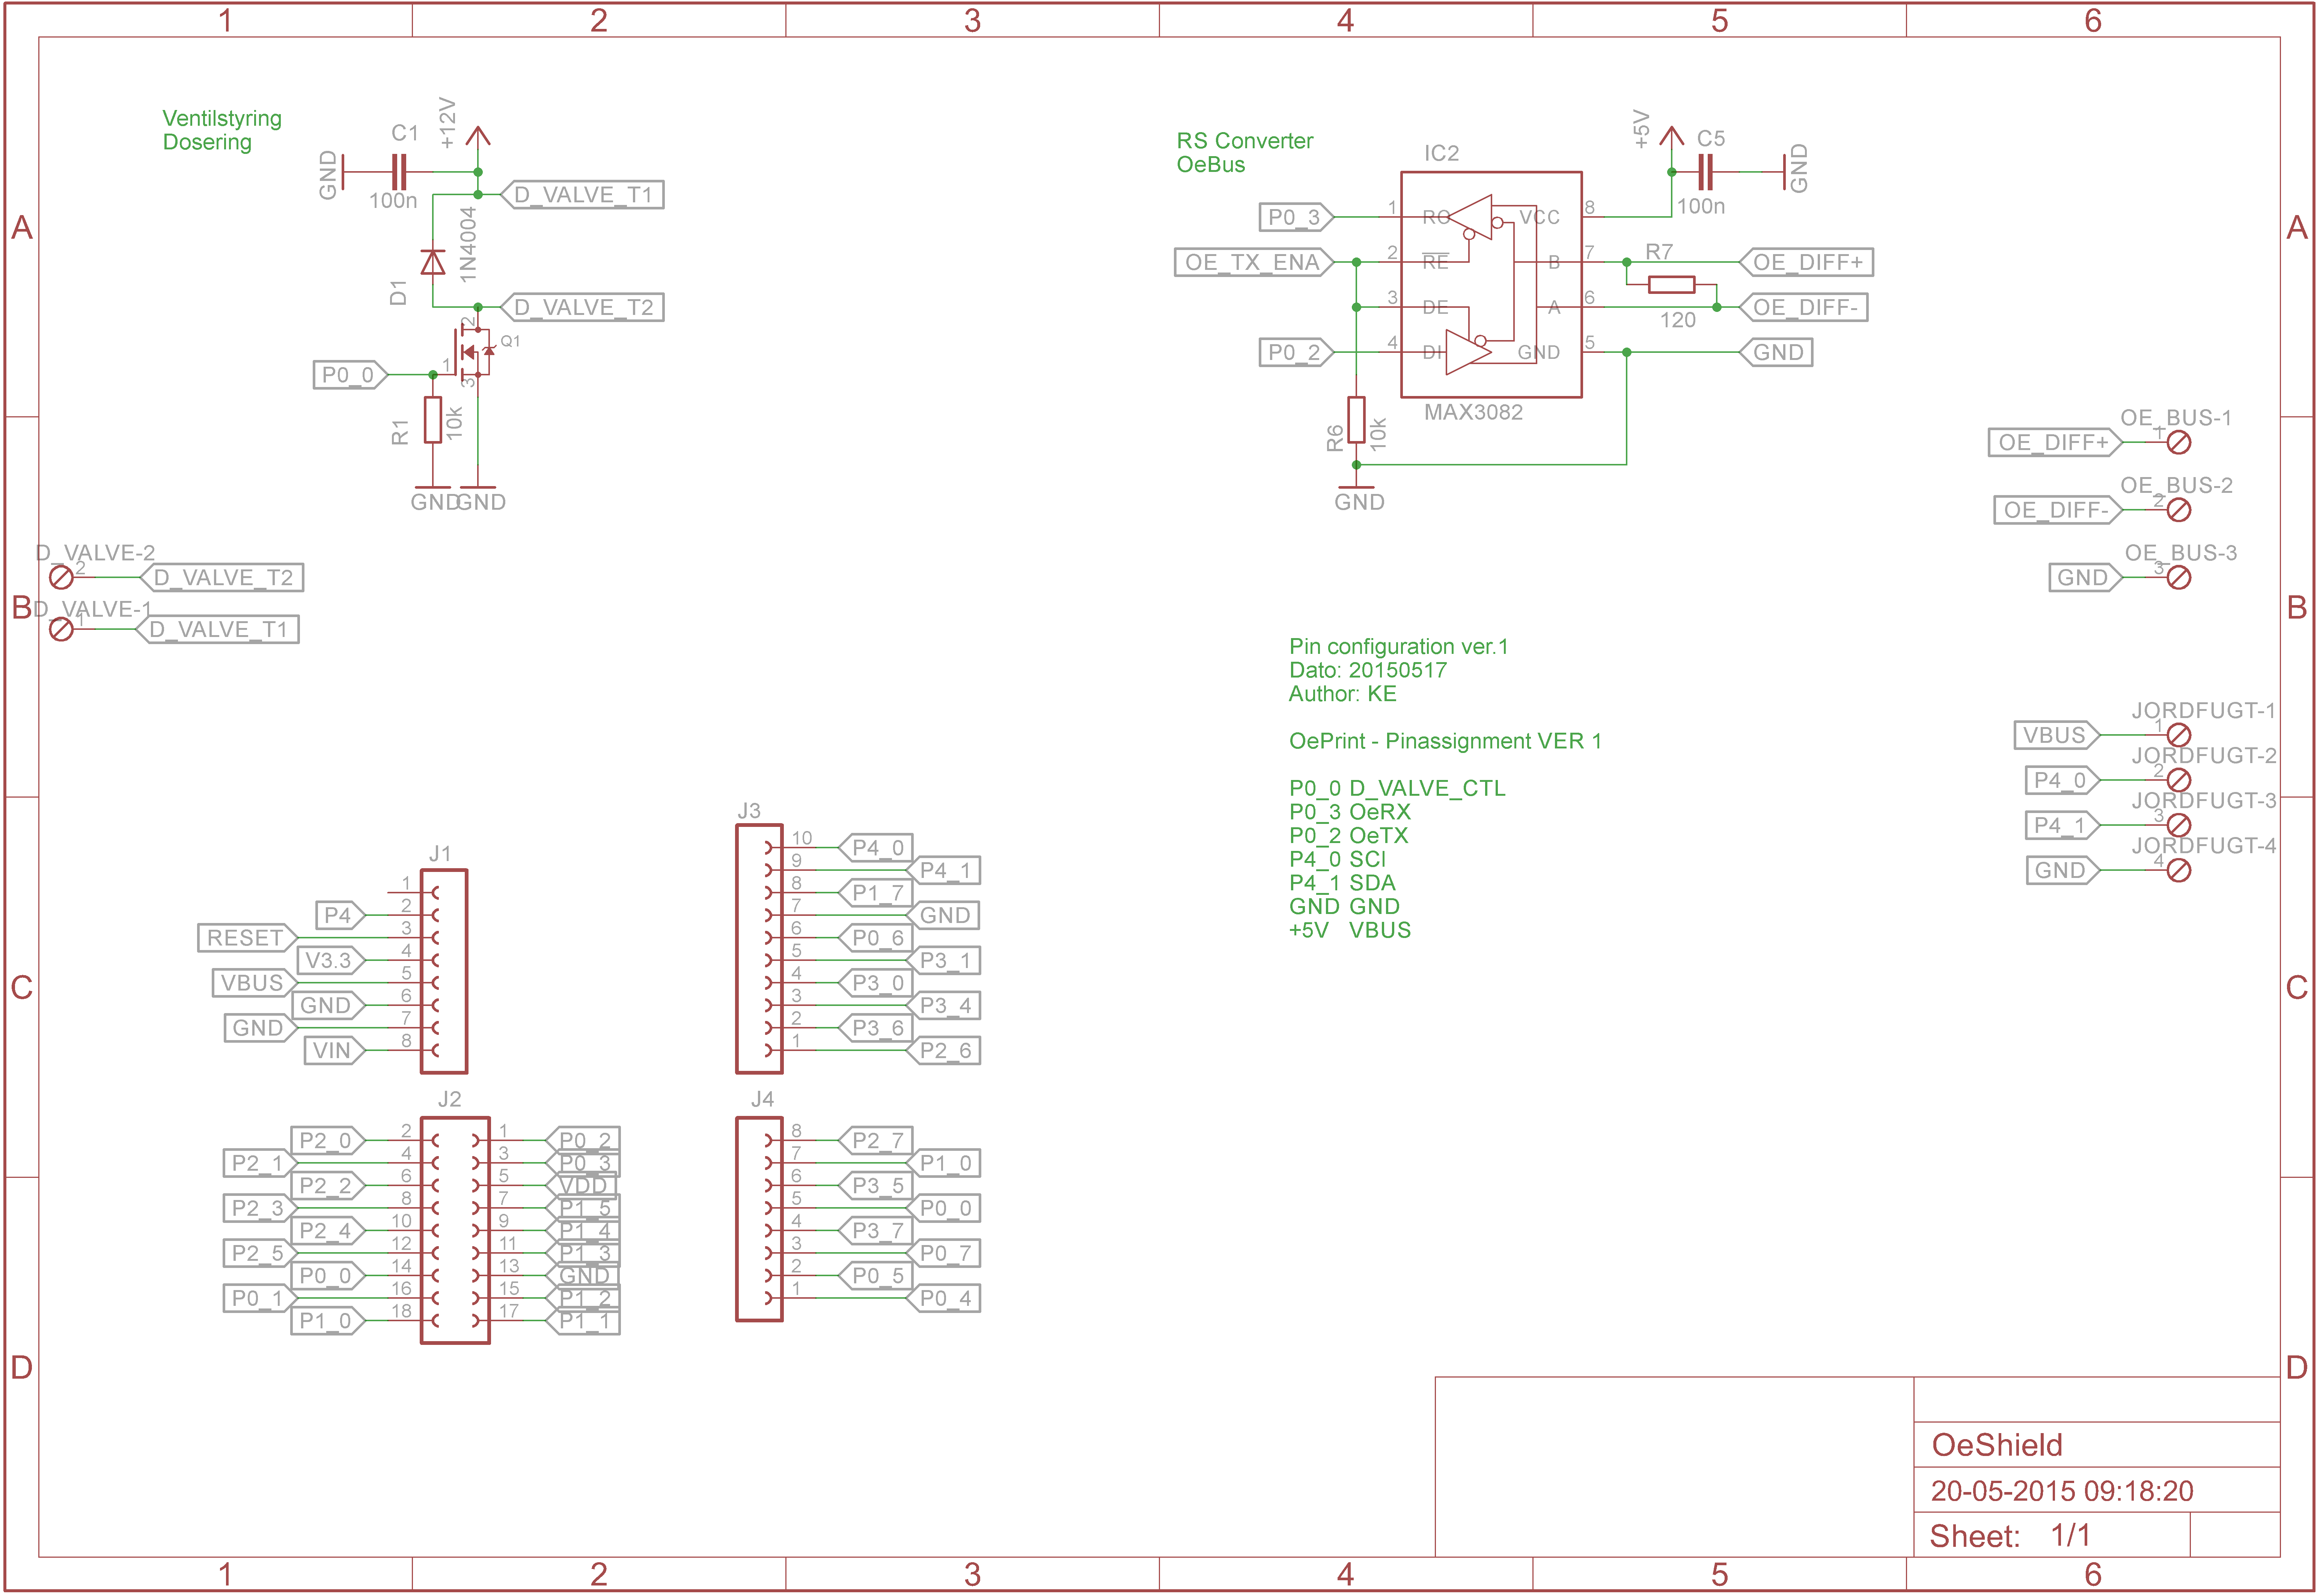
\includegraphics[scale=1]{../Hardware/Shields/Screenshots/OeShield}
	\caption{Screenshot: Det færdige ØShield}
	\label{screenshot:OeShield}
\end{figure}

\fxnote{Siden med ØShield-diagram skal være A3}


\newpage
\subsection{PiShield}

Ligeledes oprettes der et shield til Rasparry Pi'en. Dette shield indeholder følgende komponenter: 

\begin{description}
 \item[•] RS-konverter til karBus
\end{description}

Printet designes på samme måde som de 2 forrige, og det færdige print ses på på fig.\ref{screenshot:PiShield}, s.\pageref{screenshot:PiShield}.

\newpage
\begin{figure}[H]
	\centering
	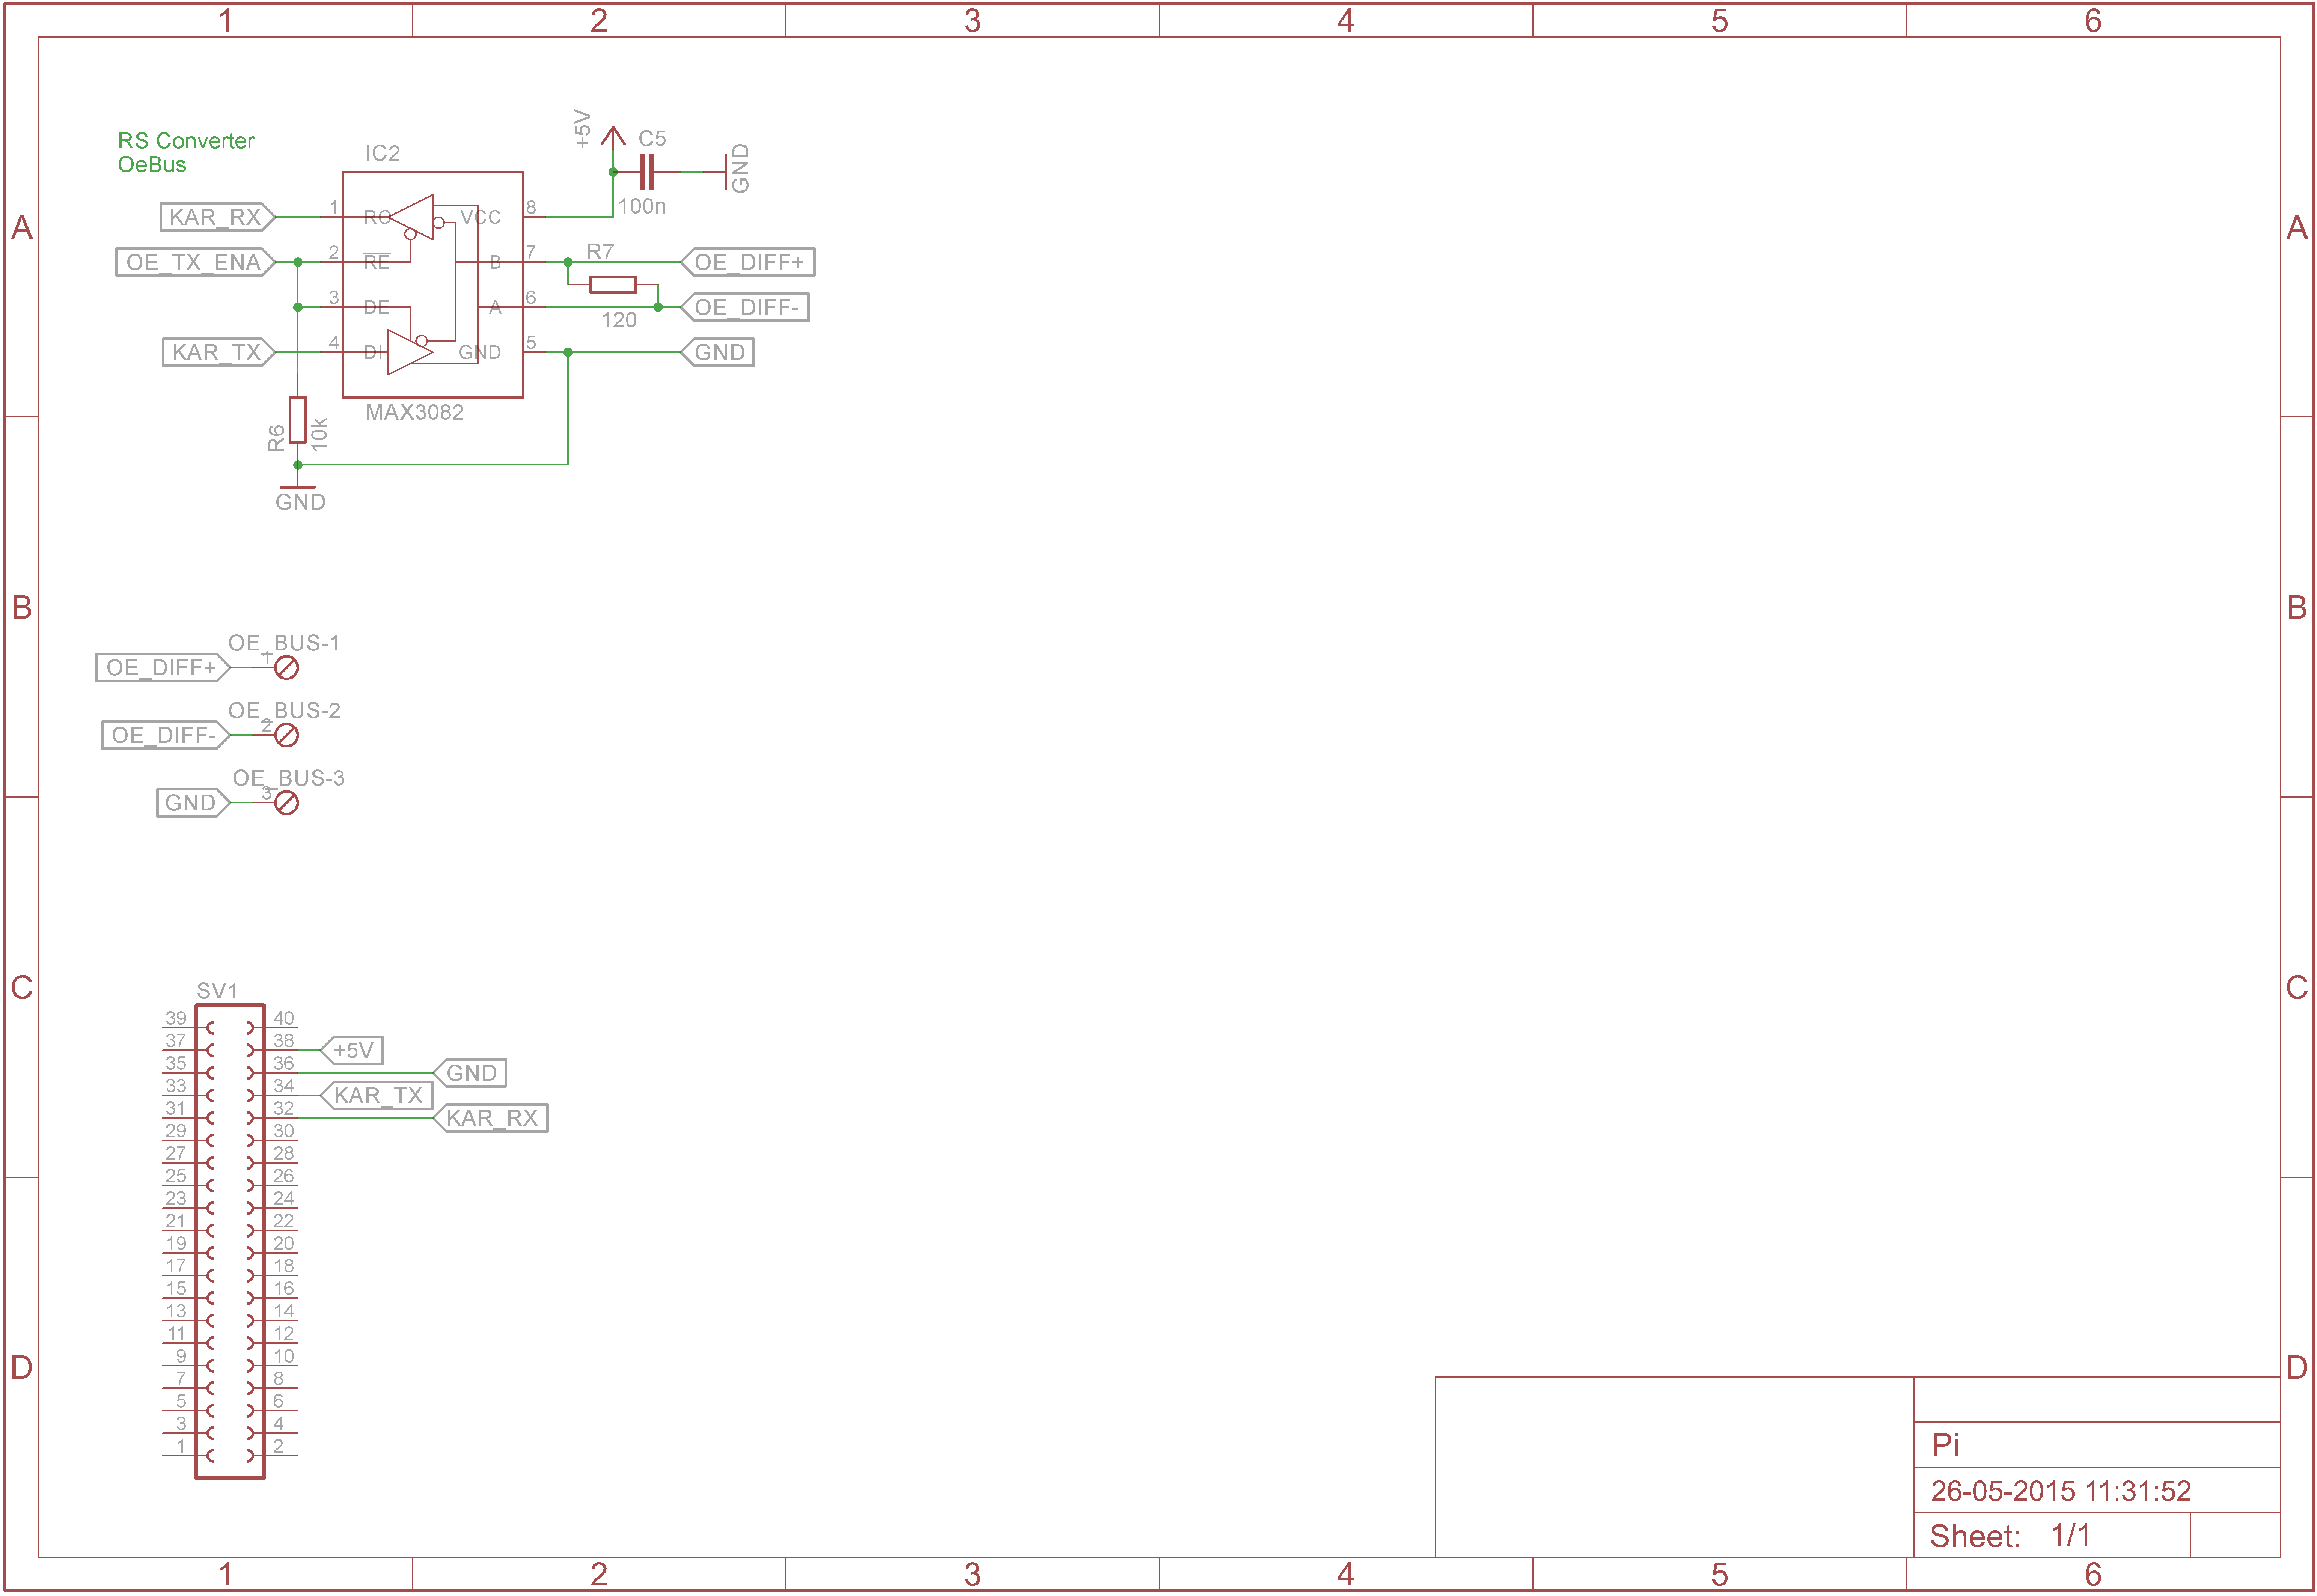
\includegraphics[scale=1]{../Hardware/Shields/Screenshots/PiShield}
	\caption{Screenshot: Det færdige ØShield}
	\label{screenshot:PiShield}
\end{figure}

\fxnote{Siden med PiShield-diagram skal være A3}

\newpage
\subsection{Printlayout}
På baggrund at disse schematics designes de 3 boards og deres printbaner lægges ud. Her tages der hensyn til følgende: 

\begin{description}
 \item[•] Hvilken strøm der løber i banen
 \item[•] Hvilken type signal der løber i banen
 \item[•] Kritiske afstande i layoutet
\end{description}

Standard tykkelsen af en printbane er 0.035 mm, og det giver en bredde på bane på 0,115 mm hvis der skal løbe 500 mA, dette er denne strøm der løber i ventiler, derfor vælges banebredden som standard til denne værdi. 
Printbanen fra forsyning til pumpen, trækkes dog 3A max, derfor vælges banebredden her til 1.37 mm. \newline
Derudover løber et PWM-kontrolsignal til pumpen på 3,5kHz, dette skaber en del støj, hvorfor denne bane bør isoleres så meget som muligt fra specielt ventilerne.\newline
Bords'ne er pt. ikke færdigdesignet, hvorfor der ikke foreligger billeder heraf. 
 